\newpage
Моя задача на данный семестр . \\
\begin{enumerate}
%\item сбор и анализ истории переписки мессенджеров;
\item преобразование собранной информации в читаемый вид;
\item добавление новых функций к уже имеющимся.
\end{enumerate}
Для упрощения разобьем задачу, на подзадачи
\begin{enumerate}
\item Создание веток(branch), и распределенная работа программистов. 
\item Визуализация данных
\item Выбор и описание утилит для преобразования
\item XSTL
\item Показать результат
\item Функция чтения контактной книги pidgin
\item Функция сбора используемых учётных записей pidgin
\item Описание работы SAX и DOM модели разбора XML
\item Функция сбора дополнительных данных skype
\end{enumerate}
\chapter*{Создание веток(branch), и распределенная работа программистов.}
Допустим мы приступаем к задаче. которая займет больше одного дня\/недели. Разработка ПО в комманде подразумевает частое создание коммитов. Это позволяет чаще получать изменения и избегать кофликтов. 

Но если задача длинная, и мы будем коммитить полу сделанную задачу, то это будет как минимум мешать другим разработчикам, как максимум сделает проект неработоспособным.[2]

Однако не делать коммиты несколько дней тоже плохой вариант. Вот для этого и существуют другие ветки. Они позволяют нам вносить изменения, не мешаю и этом остальным разработчикам. Или же работать над несколькими ветками одновременно.

Ветка - это снимок репозитария в сделанный в прошлом, в который не попадают коммиты из основной ветки после момента создания.

В проекте использовались две ветки:
\begin{enumerate}
\item master
\item skype_to_XML
\end{enumerate}

 В ветке \"master\" велась работа по переносу проекта с модульной структуры на плагииную. \"skype_to_XML\" велась работа по расширению функционала модулей клиентов - мгновенного обмена сообщениями, и VoIP программ. Велась работа по ознакомлению с языком разметки xslt, с последующей генерацией отчета в xhtml, основанный, на собранных данных, хранящихся в xml.

\begin{figure}[h]
\center{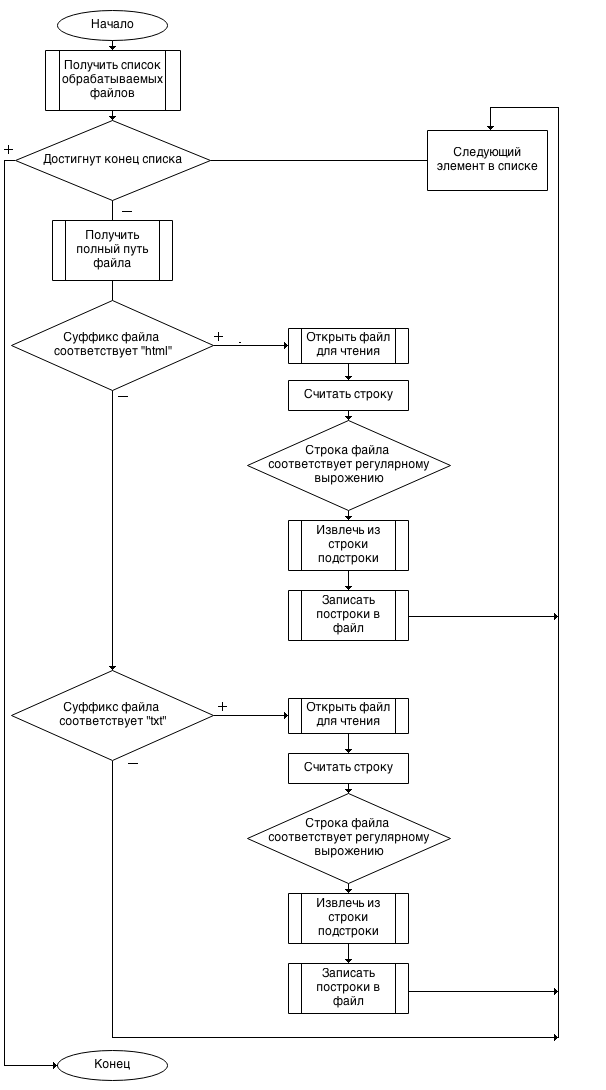
\includegraphics[width=0.5\linewidth]{Pars_pidgin_log}}
\caption{Результат работы git branch}
\label{pic:branch_project}
\end{figure}

\chapter*{Визуализация данных}
Визуализация собранной информации очень важный момент создания подобного рода комплексов, т.к. это является главной задачей нашего ПО. 

Список возможных вариантов конвертации XML
\begin{enumerate}
\item CSV
\item HTML
\item TXT
\item SQL

\item PNG
\item И многое другое...
\end{enumerate}
Из рассматриваемого списка удобным для восприятия, хранения структурированной информации и 
програмно-независимым%тут я имел в ввиду то что html можно посмотреть на любом компе, без спец програм.
оказался - HTML.
\chapter*{Выбор и описание утилит для преобразования}

XML можно хранить виде БД, а затем выводить записи БД в виде веб-страниц, используя к примеру PHP. Возникает вопрос, зачем мы храним данные в промежуточном формате XML, если в результате данные хранятся в БД. Работа в таком формате займет большее время, и сложнее ко всему. Для прямого преобразования XML в XHTML, мы можем воспользоваться языком преобразования XSLT. 
\chapter*{XSTL}
\\XSLT (eXtensible Stylesheet Language Transformations) — это расширяемый язык стилей для преобразований, который использует для описания преобразований структуры документов.[1]
\\Хотя XSLT не позиционируется, как язык запросов для XML, можно смело сравнить есго с языком SQL, в котором определяются запросы к реляционным базам данных.[1]

При применении таблицы стилей XSLT, состоящей из набора шаблонов, к XML-документу образуется конечное дерево, которое может быть сериализовано в виде XML-документа, XHTML-документа (только для XSLT 2.0), HTML-документа или простого текстового файла. Правила выбора (и, отчасти, преобразования) данных из исходного дерева пишутся на языке запросов XPath.
XSLT имеет множество различных применений, в основном в области веб-программирования и генерации отчётов. Одной из задач, решаемых языком XSLT, является отделение данных от их представления, как часть общей парадигмы MVC (англ. Model-view-controller). Другой стандартной задачей является преобразование XML-документов из одной XML-схемы в другую.[3]
\chapter*{Результаты работы}

\begin{figure}[h]
\center{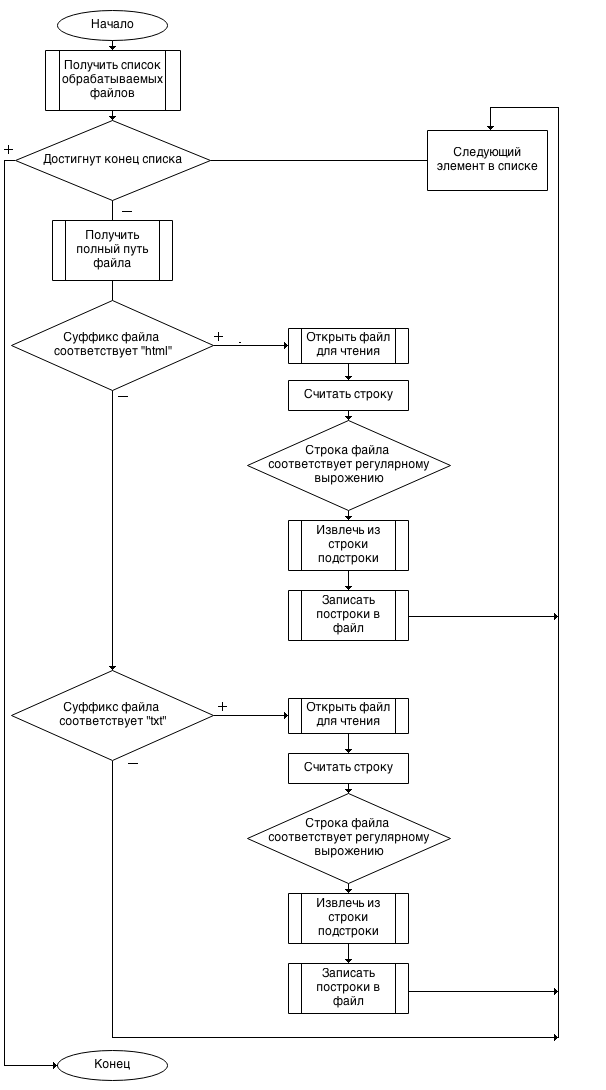
\includegraphics[width=0.5\linewidth]{Pars_pidgin_log}}
\caption{Результат заглавной генерированной страницы отчета}
\label{pic:xml_to_xslt1}
\end{figure}

\begin{figure}[h]
\center{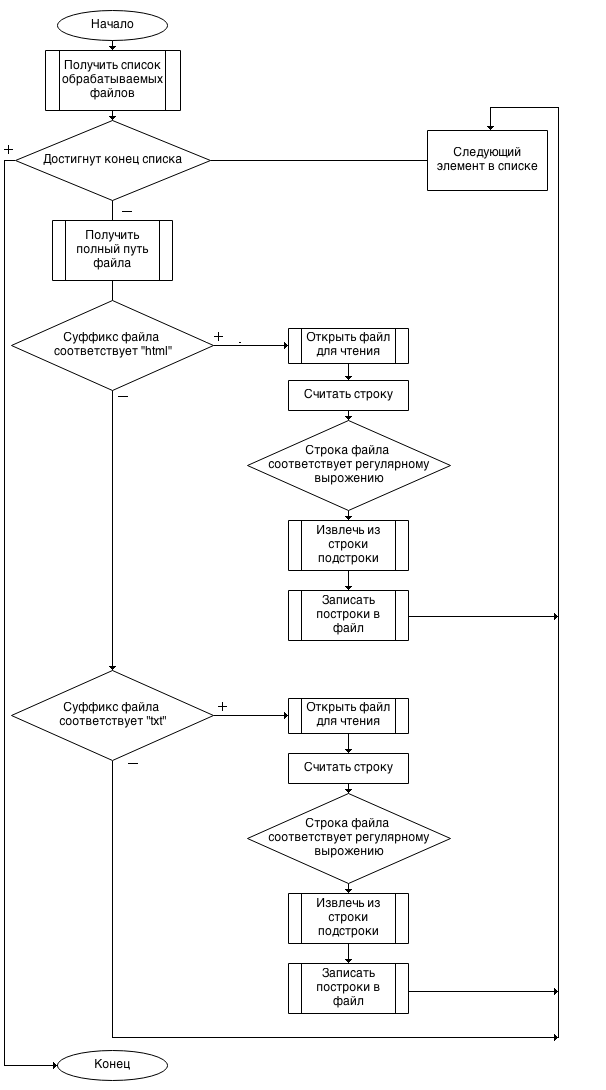
\includegraphics[width=0.5\linewidth]{Pars_pidgin_log}}
\caption{Результат сбора данных контактной книги pidgin}
\label{pic:xml_to_xslt2}
\end{figure}

\begin{figure}[h]
\center{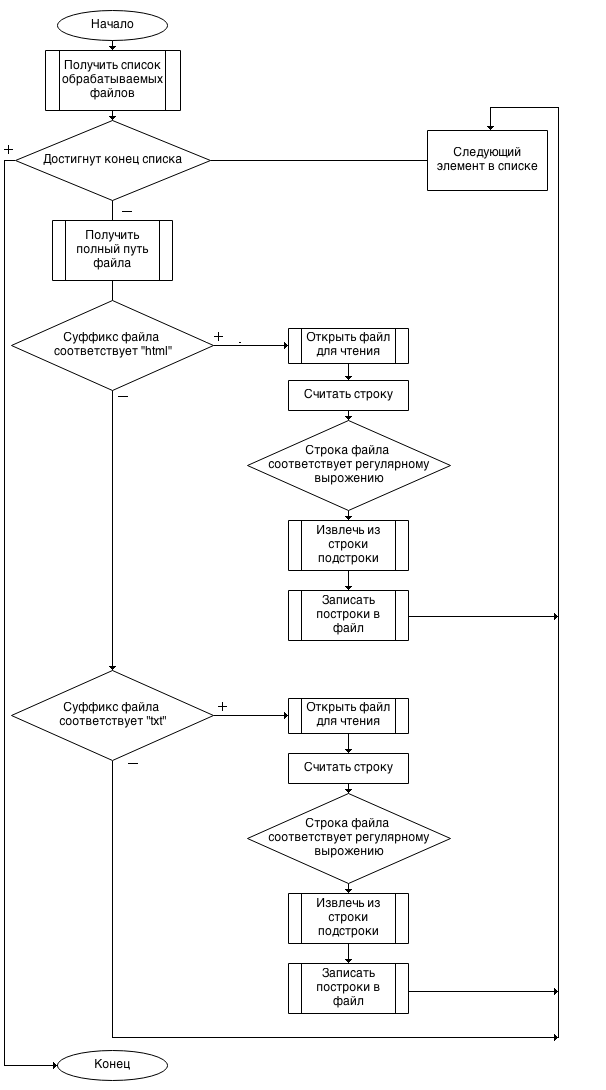
\includegraphics[width=0.5\linewidth]{Pars_pidgin_log}}
\caption{Результат сбора данных аккаунта pidgin}
\label{pic:xml_to_xslt3}
\end{figure}

\begin{figure}[h]
\center{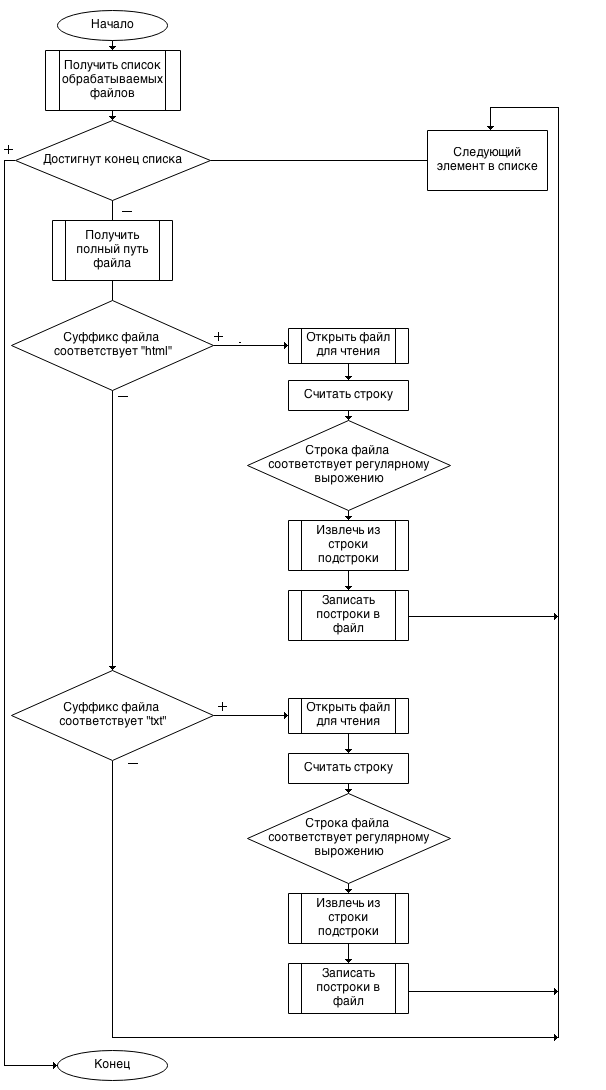
\includegraphics[width=0.5\linewidth]{Pars_pidgin_log}}
\caption{Результат сбора данных контактной книги skype}
\label{pic:xml_to_xslt4}
\end{figure}

\begin{figure}[h]
\center{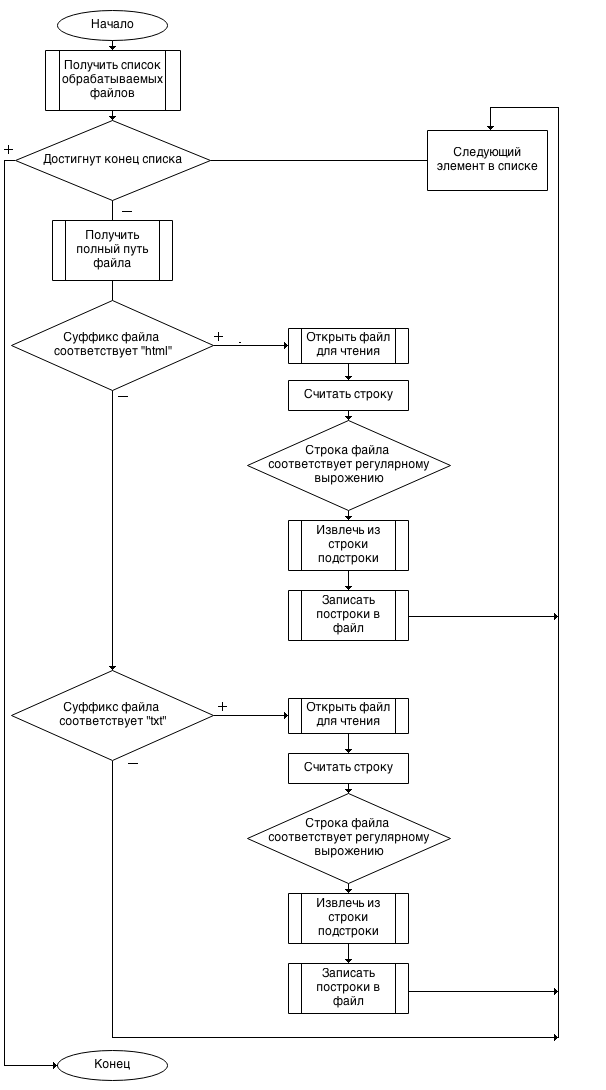
\includegraphics[width=0.5\linewidth]{Pars_pidgin_log}}
\caption{Результат сбора данных аккаунта skype}
\label{pic:xml_to_xslt5}
\end{figure}

\begin{figure}[h]
\center{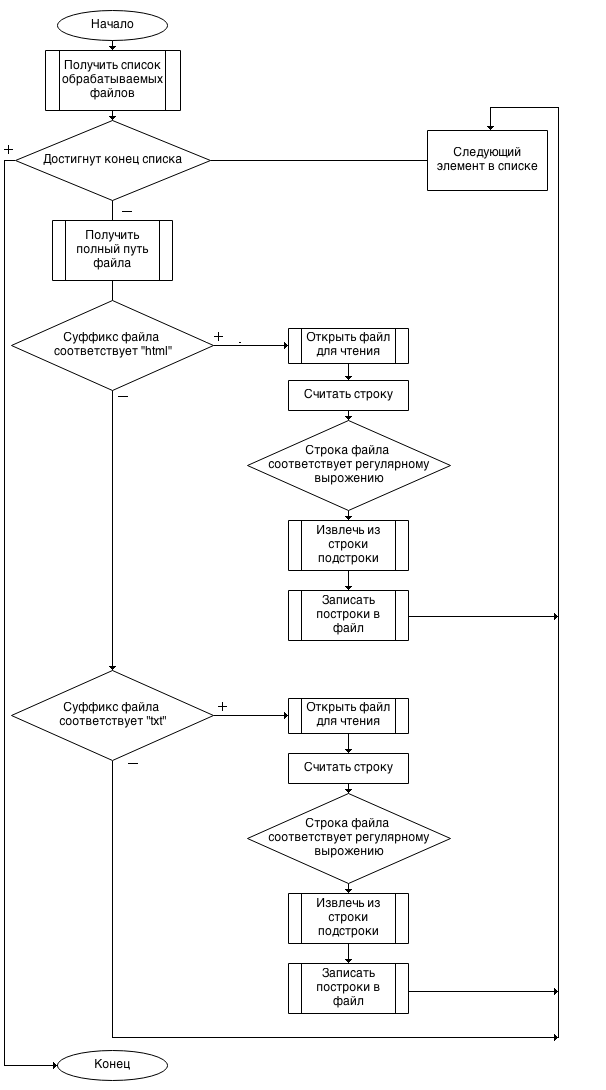
\includegraphics[width=0.5\linewidth]{Pars_pidgin_log}}
\caption{Результат сбора данных звонков skype}
\label{pic:xml_to_xslt6}
\end{figure}

\begin{figure}[h]
\center{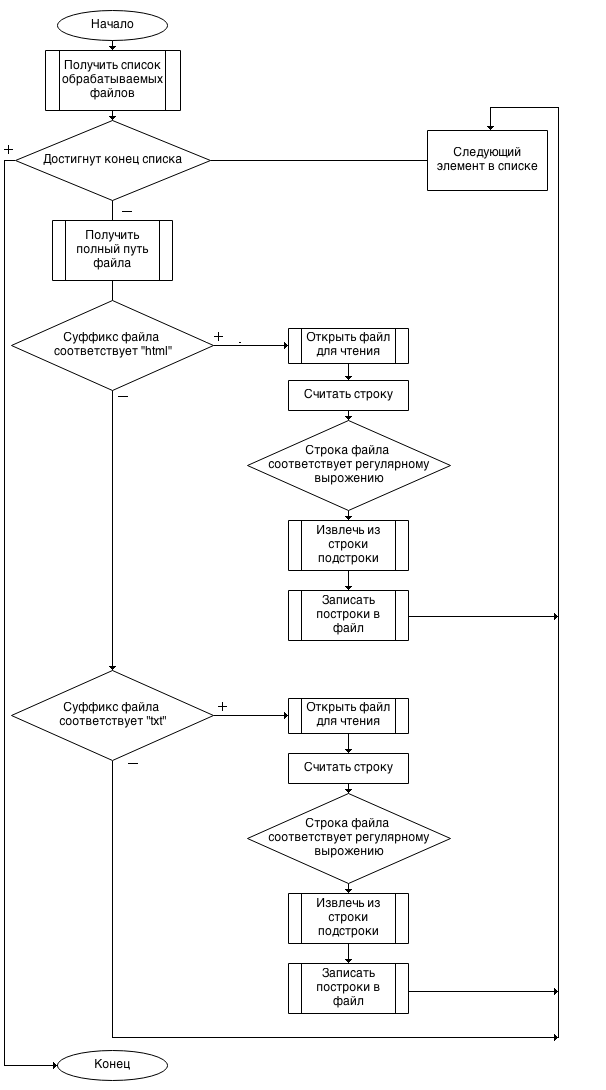
\includegraphics[width=0.5\linewidth]{Pars_pidgin_log}}
\caption{Результат сбора установленного ПО}
\label{pic:xml_to_xslt7}
\end{figure}

\chapter*{Описание работы SAX и DOM модели разбора XML}

SAX расшифровывается как Simple API for XML, что означает буквально \"Простой прикладной интерфейс программирования для XML\"

SAX (англ. «Simple API for XML») — способ последовательного чтения/записи XML-файлов.

Всё, что делает SAX-парсер, это сообщает вызвавшему приложению о встреченных распознанных элементах XML-разметки или о встреченных ошибках. Связь парсера с вызывающим приложением, как правило, осуществляется посредством функций обратного вызова.

DOM (от англ. Document Object Model — «объектная модель документа») — это не зависящий от платформы и языка программный интерфейс, позволяющий программам и скриптам получить доступ к содержимому HTML, XHTML и XML-документов, а также изменять содержимое, структуру и оформление таких документов.
[1]%Дернуть из книги%
\chapter*{функция чтения используемых аккаунтов и контактной книги pidgin}
Интересующие нас контактная книга находятся в %путь написать тут%
в файле blist.xml, используемые аккаунты хранятся в файле accounts.xml.
\\Оба файла имеют идентичную древовидную структуру, которая начинается в \"корне\" и разветвляется до \"листьев\", как и положено в XML документе.
\begin{figure}[h]
\center{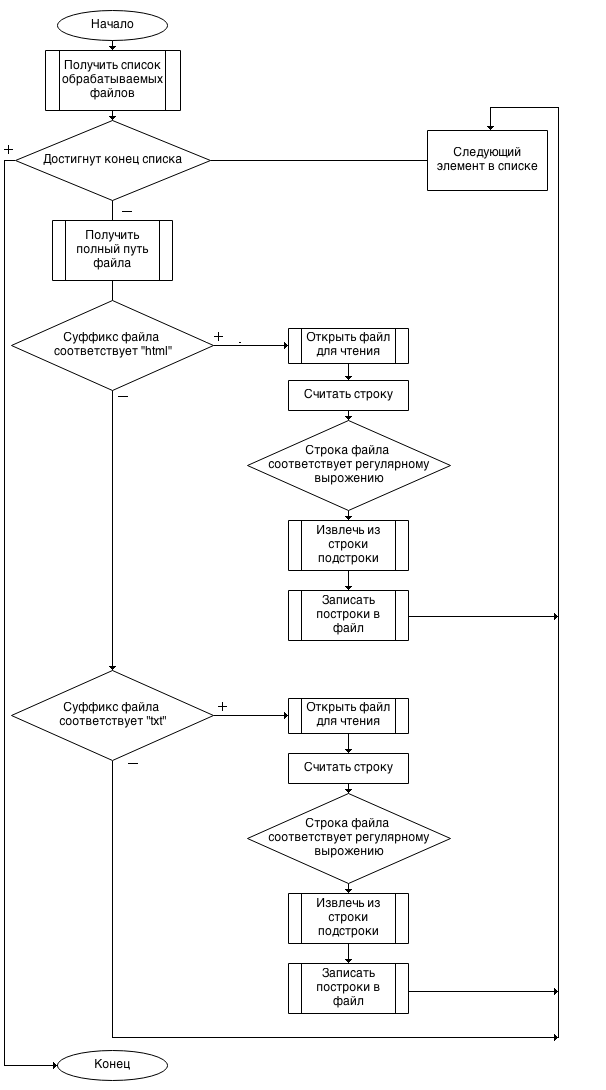
\includegraphics[width=0.5\linewidth]{Pars_pidgin_log}}
\caption{Граф построенный по данным accounts.xml}
\label{pic:xml_to_xslt7}
\end{figure}

Для разбора данного файла использовалась модель SAX. Реализованная в библиотеке QT, в классе QXml. При проходе по дереву XML мы реагируем на события[4]:
\item Старт документа
\item Старт элемента
\item CDATA (анг. Character Data) Символьный тип данных
\item Комментарии
\item Конец документа
\item Конец элемента
\item Ошибка чтения

При проходе парсера по файлу мы реагируем на нужные нам элементы, атрибуты и прочее. Затем данные вычитываются, и сохраняются в XML отчет.
\chapter*{функция сбора дополнительных данных skype}
К имеющемуся списку функций работы с логами VoIP skype в этом семестре добавилось. Функция извлечения информации о аккаунтах, когда-либо авторизовавшихся на данном компьютере. Т.е при авторизации на компьютере создается лог этого пользователя в виде main.db. Помимо прочего этот файл содержит в себе информацию о используемом акаунте. Полное имя, почту, ... которое извлекается при запуске таска.



Список использованной литературы:
1 -  Технология XSLT Валиков Алексей 2002г. ссылка http://www.e-reading.ws/book.php?book=1016301
2 -  GIT Pro Глава 3.1 Scott Chacon 2014г. ссылка 
3 -  XSLT - статейка на вики.
4 -  Документация QT: Раздел XML Reader.